% !TEX root =  CurvedFoldedDogs.tex

\section{Folding crease patterns} \label{sec:folding}
In this section we explore the different ways one can fold a given crease pattern. Our result is a discrete combinatorial characterization for the local existence of a fold in a piecewise DOG.

%Two intersecting developable surfaces can be flattened along their intersection if the intersected curve have the same geodesic curvature on both surfaces. 
\subsection{The smooth and combinatorial degrees of freedom around a single curved crease}
Straight creases are rather boring, mathematically speaking. Straight lines can only be folded as in classical origami, i.e., by keeping them straight \cite{demaine_lens}. \OSH{Or Tim's comment -- if the line becomes curved, it means that we have a ``double cover'', i.e., we folded 180 degrees and the two sheets coincide completely now.} Hence a folding of a single straight crease can be described by a single real number representing the constant dihedral angle between the incident planes. There are far more ways, or degrees of freedom, to fold a curved crease. Let $S$ be a curved folding \OSH{folded?} deformation of a given flat configuration $S_p$; assume a crease pattern consisting of a single crease such that $S = P_1 \cup P_2$ (\figref{fig:folding_combinatorics} left). Let $\Gamma(t) = P_1 \cap P_2$ be the 3D crease curve and $\gamma(t)$ its flattening in $S_p$ \OSH{add this notation to Katja's figure}. Let $\kappa(t)$ be the curvature of $\Gamma(t)$ and $\kappa_g(t) = \kappa(t) \cos(\alpha(t))$ be its geodesic curvature,  which is the curvature of the planar curve $\gamma(t)$ \OSH{who is $\alpha(t)$?}. Assume that the curve is  bent further in space, i.e., $\kappa(t) > \kappa_g(t)$. Then the tangent planes of $P_1$ and $P_2$ form an angle of $\alpha(t) \neq 0$ \OSH{$2\alpha$?} with the osculating plane of $\Gamma(t)$ \cite{more_on_paper,duncan_folded}. Since $P_1,P_2$ are $C^2$,  there are four options for a consistent choice of a family of tangent planes along each side of the crease $\Gamma(t)$. Two of these four options correspond to a folding (i.e., tangent discontinuity) by choosing one family tangent planes along $\Gamma(t)$ for $P_1$ and the other for $P_2$ (see \figref{fig:folding_combinatorics}).
\begin{figure} [h]
	\centering
	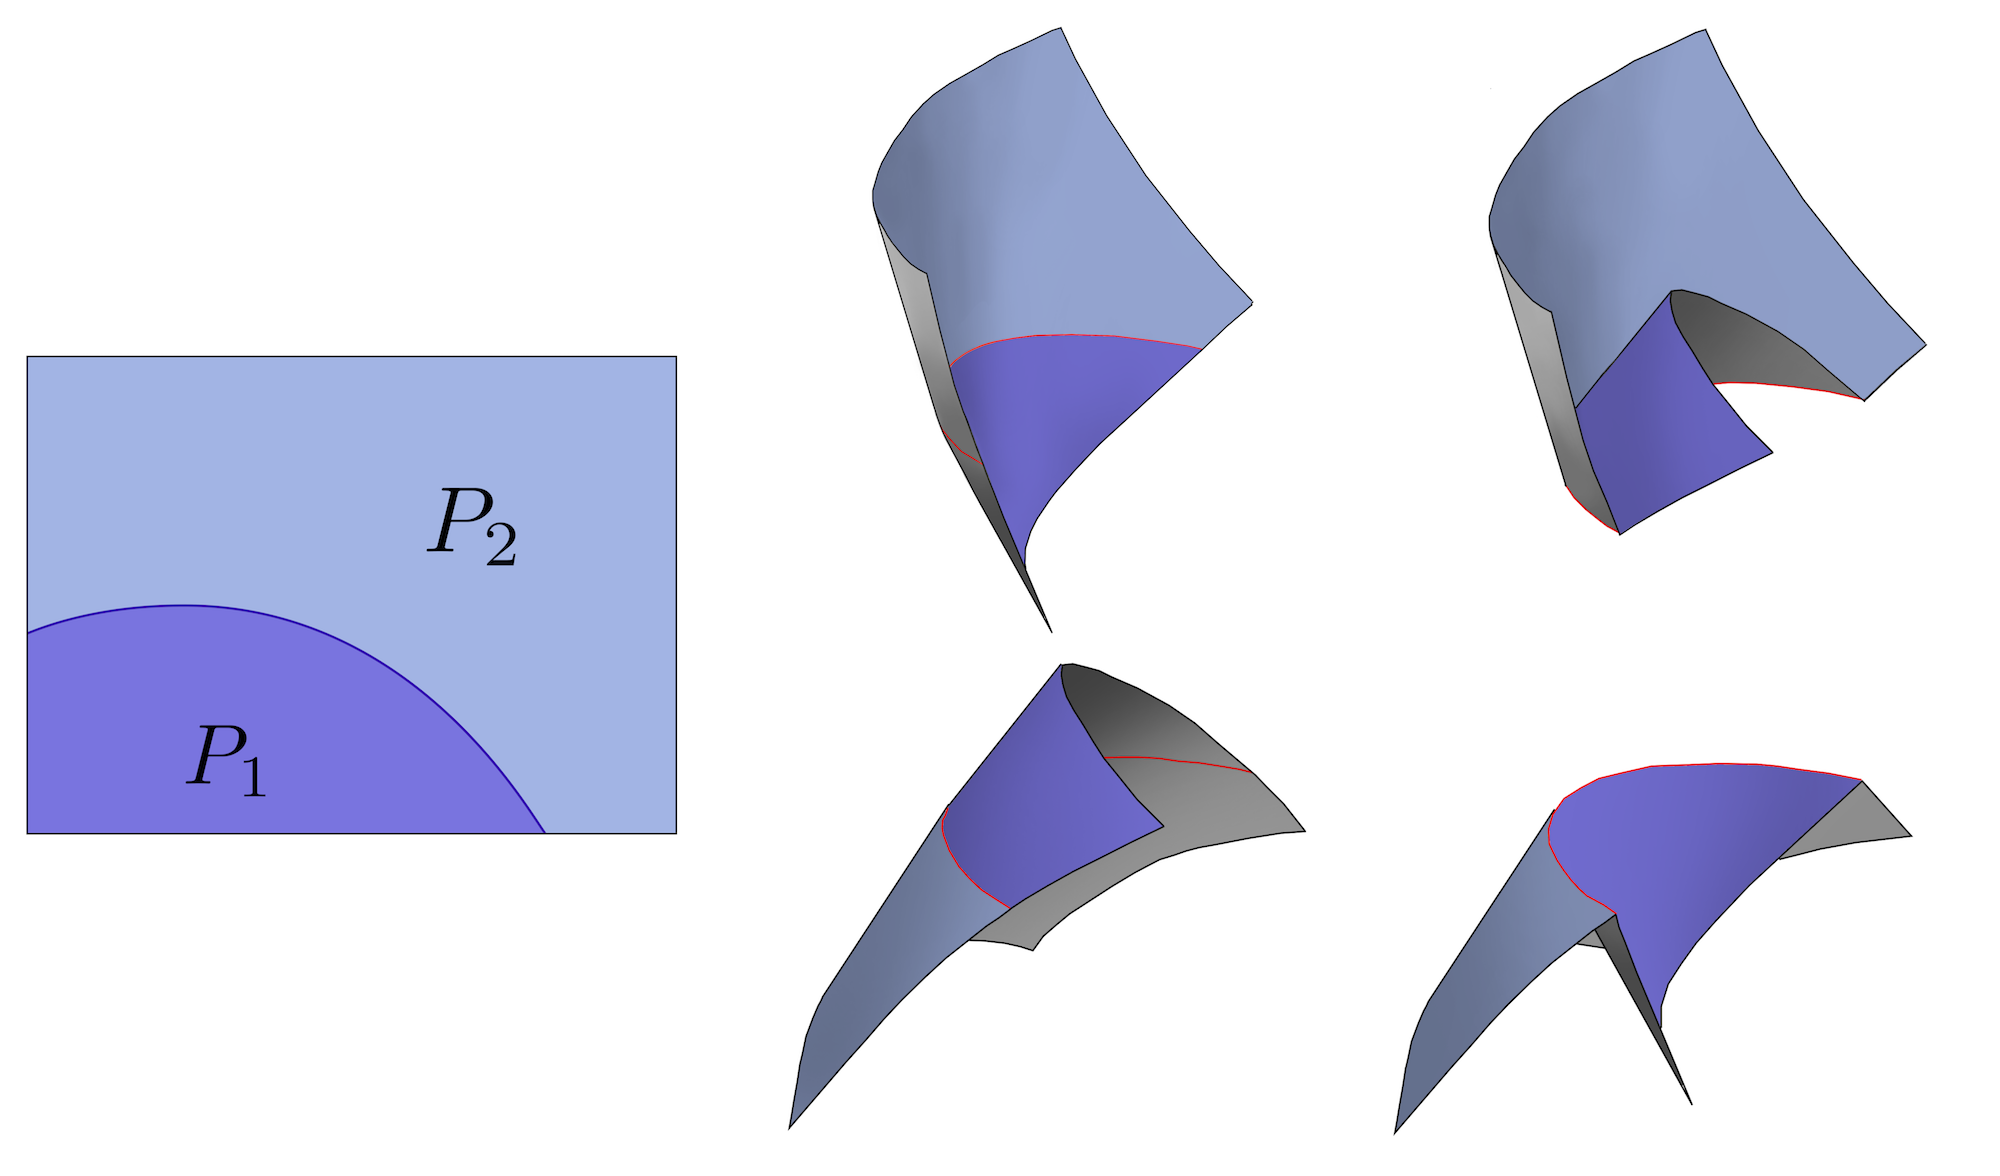
\includegraphics[width=\linewidth]{figures/curved_fold_through_curve.png}
	\caption{The combinatorial degrees of freedom in curved folding. If a crease pattern of a curved folded surface (left) is isometrically folded such that a given curve lies in some configuration in $\R^3$, then there are only two smooth surfaces $S_1,S_2$ that isometrically flatten into the crease pattern (center). One can also choose a different surface for each patch $P_1,P_2$, resulting in two other curved folded surfaces (right). \OSH{In the text we don't use $S_1, S_2$ notation anymore, you always use $P_1,P_2$, also for 3D. Should we use $P_{p,1}, P_{p,2}$ for the flat configuration of the patches, or do you want to go back to $P$ for flat and $S$ for non-flat?}}
	\label{fig:folding_combinatorics}
\end{figure}

Given this combinatorial degree of freedom, the curvature and torsion \OSH{it's the first time you mention torsion, I would explicitly explain how it comes in - not very clear} of the curve $\Gamma(t)$ locally determines the shape of the surface, since the rulings of each developable part are the intersections of the developable's tangent planes, and the rulings emanating from the curve $\Gamma(t)$ in each developable $P_1,P_2$ extend to their boundary \cite{spivak,more_on_paper} \OSH{why is this important? what if there is a cone (rulings meet in a singularity)? sorry, confused}. The ruling patterns of the surfaces change as well \OSH{as what?} during the deformation \OSH{deformation of what?}, making modeling of such surfaces using discrete ruling based representations challenging (see \figref{fig:rulings_problem_curve}). The angle between the different tangent planes on each surface, $2\alpha(t)$, is called the folding angle, which by construction is bisected by the osculating plane of the curve. Unlike the case of a straight crease, the folding angle generally varies along the curve. \OSH{the ruling based methods discussion is maybe a bit out of place?}

To summarize, the shape of a surface $S$ that is folded along a single curved crease $\Gamma(t)$ can be locally described by two \textit{real functions} $\kappa(t),\tau(t)$ \OSH{$\tau$ was not introduced yet} and one combinatorial parameter distinguishing between four possible surfaces, two of which are folded (see \figref{fig:folding_combinatorics}).
 
%(there's the cone singularity case where a curved fold is more local (as focused on the cone point) but I think this requires the curve to be C^1.. should mention it?

\subsection{The combinatorial parameters of multiple creases}
The previous analysis explains the local behavior of curved folding around a single curve. Understanding crease patterns globally still remains a challenge. In essence, deforming one patch propagates a global deformation of the patch on the other side of the crease, a process that depends on the fixed creases \OSH{you mean locations of creases?} and the possibly changing ruling patterns. When there are multiple creases, the propagation dictates the shape of other patches. The process becomes more complicated when some creases intersect, due to compatibility constraints (see \figref{fig:multiple_crease_patterns}). 

\begin{figure} [h]
	\centering
	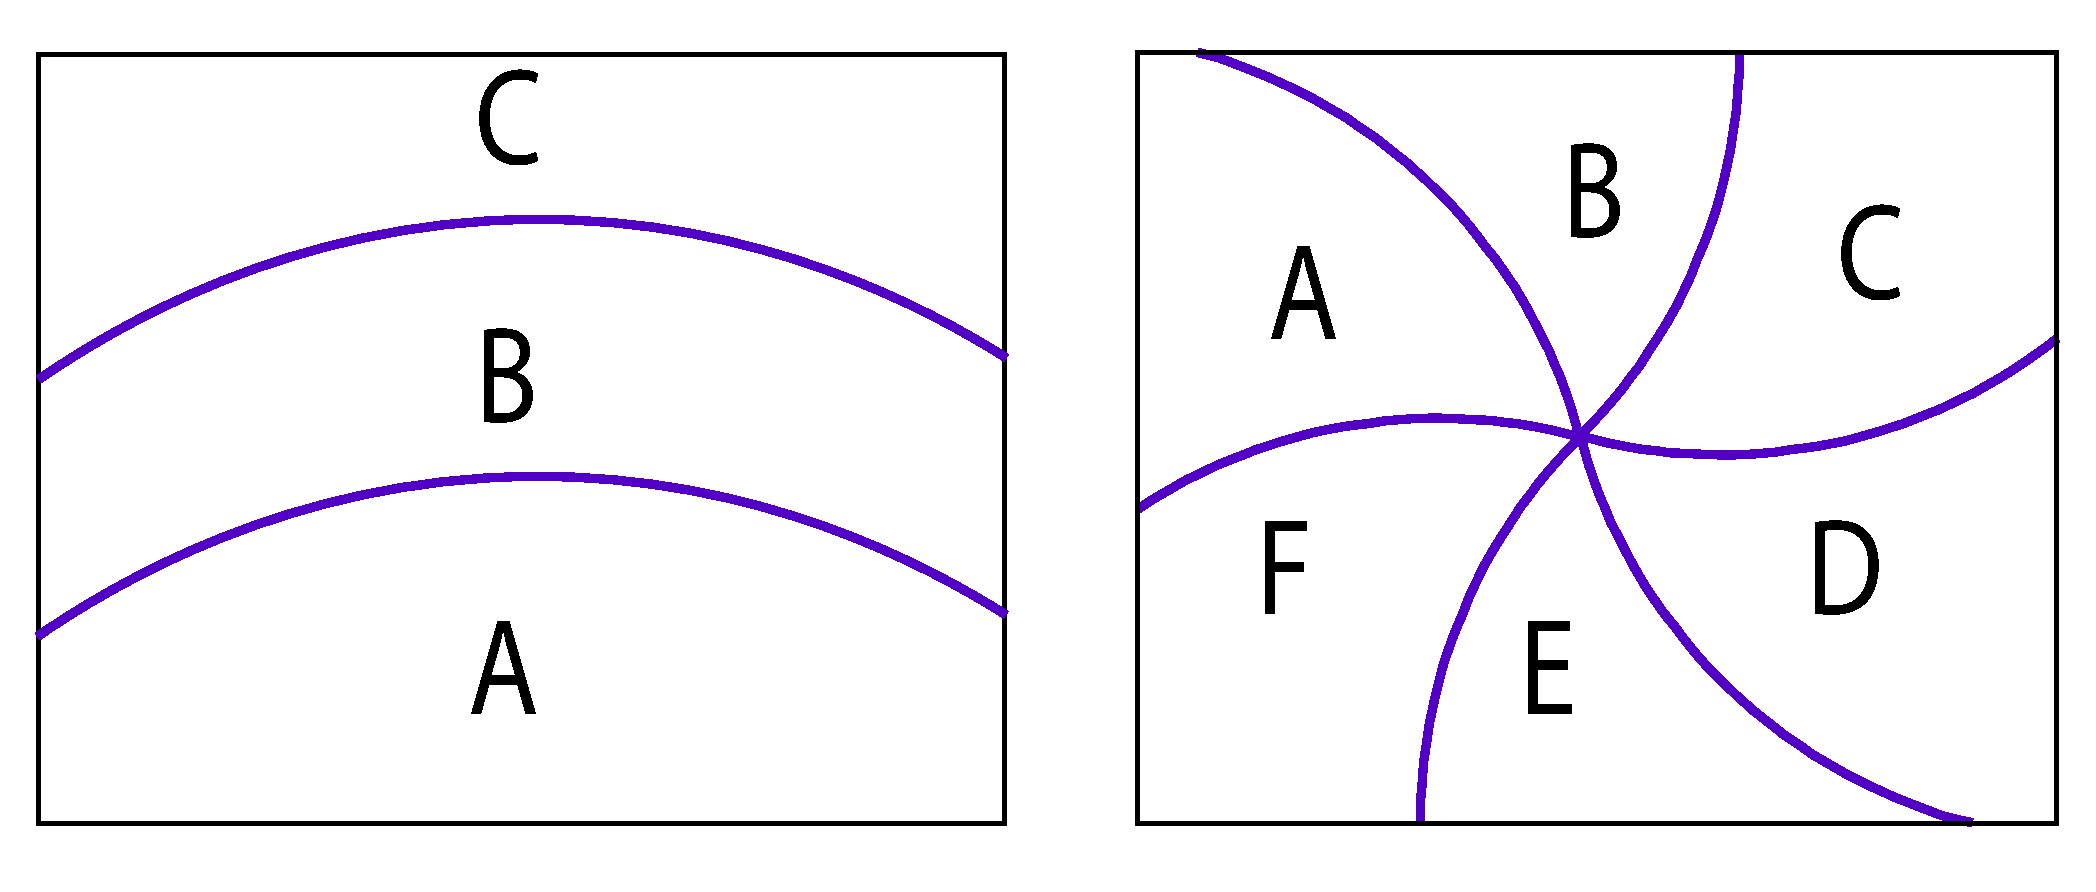
\includegraphics[width=\linewidth]{figures/multiple_crease_patterns}
	\caption{Propagation of constraints in crease patterns. Down: Crease patterns. Up: Curved folding of the crease patterns. Left and Center: A deformation in the patch $P_1$ dictates most of the shape of the patch $P_2$ which in turn dictates most of the patch of $P_3$. The propagation of deformation is generally global, and depends on the directions of the rulings. In these cases one can choose a mountain/valley assignment for one fold, which already determines the M/V assignment of the next fold (left: valley-mountain, center: valley-valley). Right: In more complicated crease patterns, for instance those with a vertex, the process is more complicated as there are also some compatibility conditions the patches need to satisfy. }
	\label{fig:multiple_crease_patterns}
\end{figure}

Generally speaking, one may be able to choose between four different configurations of the surface at one crease, but this choice already fixes the patch shape for nearby creases. The combinatorial degrees of freedom that remain are whether each crease is folded or not (see \figref{fig:folded_and_not_folded}). The difficulty in modeling folding of a planar surface stems from the fact that these combinatorial choices often need to be enforced at the beginning of the folding process, as explained by the following theorem.% combinatorial degree of freedom is often only available at the start of a deformation of a flat surface, as detailed in the following lemma:

\begin{theorem}\label{Thm:curved_folding_open_condition}
Let $S(t)$ be a curved folding flow and let $p(t_k)$ be a point on a curved crease of $S(t)$ lying on two patches $P_1,P_2$ at a given time in the flow, $t=t_k$. If $p(t_k)$ is not a planar point on $P_1$ (or equivalently on $P_2$), then there exists an $\epsilon > 0$ such that one of the following holds:
\begin{enumerate}
	\item $\ S(t)$ is folded at $p(t)$ for every $t \in (t_k-\epsilon, \ t_k+\epsilon)$;
	\item $\ S(t)$ is \emph{not} folded at $p(t)$ for every $t \in (t_k-\epsilon, \ t_k+\epsilon)$.
\end{enumerate}
\end{theorem}
\begin{proof}
Let $\kappa(p(t))$ be the crease curvature at the point $p(t)$, and let $\kappa_g(p(t)) = \kappa(p(t))\cos\alpha(p(t))$ be the crease's flattened (geodesic) curvature \OSH{, where $\alpha(p(t))$ is...}. If $\alpha \neq 0$, the claim follows from the discontinuity of the two possible tangent planes at $p(t)$: a folding corresponds to a different choice of the tangent planes, both forming an angle of $2\alpha(p(t))$ with each other, and any small continuous deformation cannot move from a folded to a non-folded configuration or vice-versa. Finally, the non-planarity of $p(t_k)$ implies $\alpha(p(t_k)) \neq 0$, since $\alpha(p(t_k)) = 0$ would mean that the normal curvature of the crease curve is $0$ and therefore the tangent of the crease curve is parallel to the ruling direction (see inset). But by Lemma 12 and Corollary 16 in \cite{demaine_lens} this implies that the curve has a kink at  $p(t_k)$, contradicting the fact that the deformation flow $S(t)$ is $C^2$ when restricted to the patches $P_1$ or $P_2$.
\end{proof}
\setlength{\columnsep}{8pt}%
\begin{wrapfigure}{r}{0.3\linewidth}
  \centering
  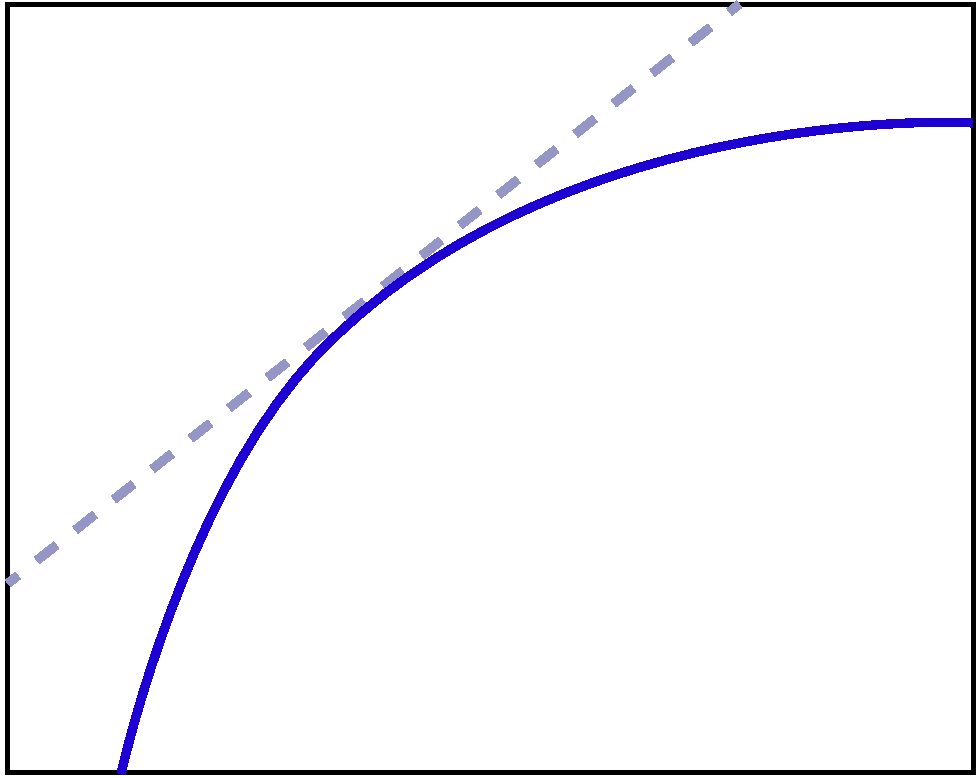
\includegraphics[width=\linewidth]{figures/ruling_tangent_to_a_curved_fold}
%  \caption{\label{fig:cone_from_curve} A local representation of a developable surface through a curvature line curve $\gamma(s)$, and orthogonal rulings emanating from it.}
\end{wrapfigure}

Therefore it is impossible to fold a crease point that is non-planar. On a non-planar point that is not folded, any small deformation keeps it that way. Folding can only happen after flattening the point, and if the surface is already folded, any small deformation keeps it folded. Thus, the decision to fold or not to fold can only be done when the crease points are planar, while no extra care needs be taken if the crease is already folded. With this in mind, we note the following observation.

\begin{theorem}\label{Thm:supporting_plane}
A non-planar curved crease point on a curved folded surface $S$ is folded if and only if the osculating plane of the crease curve at that point is locally a supporting plane for the surfaces $P_1,P_2$ intersecting at the point (see inset \OSH{Can you make the surface in the inset look less like double-cover, i.e., a bit less sharp fold?}).
\end{theorem}
\setlength{\columnsep}{8pt}%
\begin{wrapfigure}{r}{0.3\linewidth}
  \centering
  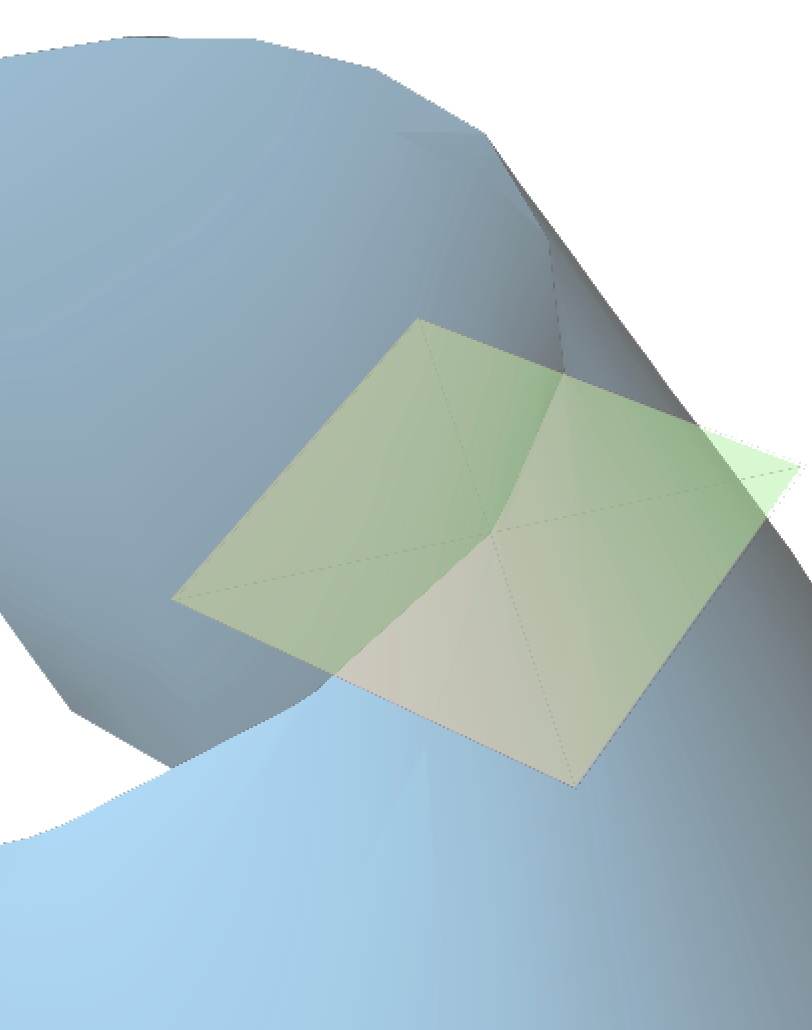
\includegraphics[width=\linewidth]{figures/plane_side}
\end{wrapfigure}
This follows directly from the fact that the tangent planes on both sides of a crease curve coincide if the surface is smooth there, but along a folded crease they are reflections of one another through the crease curve's osculating plane. Planar crease points along a curved crease, while not folded, still satisfy this constraint, since around these points the tangent planes are exactly the same as the osculating plane of the curve, though even the slightest surface deformation might change that. 

\subsection{Discretization}
\OSH{We saw that folding happens exactly when both sides of the surface around a crease are in the same half-space of the osculating plane of the crease curve.} We discretize this condition by constraining the tangents of the discrete parametric (grid) lines of the two DOG patches to be on the same side of the crease curve's discrete osculating plane. See \figref{fig:osc_plane_discretization} for the notation. The DOG edges intersecting the crease can be considered as discrete tangents originating at the crease points. In the notation of \figref{fig:osc_plane_discretization}, each of the two patches has its own edge ($e^1$ or $e^2$) intersecting the crease curve. In the starting, flat configuration the two edges coincide, but a folding movement creates a discontinuity along them. We denote the tangents as $t_1 = \frac{t_1}{\|t_1\|}, t_2 = \frac{t_2}{\|t_2\|}$ \OSH{you mean $t^1 = \frac{e^1}{\|e^1\|}, t^2 = \frac{e^2}{\|e^2\|}$?}. We denote the crease curve's binormal, i.e., the normal of its osculating plane, as $B = \frac{e_f \times e_b}{\|e_f \times e_b\|}$, noting that $e_f,e_b$ coincide for both patches.

\begin{figure} [h]
	\centering
	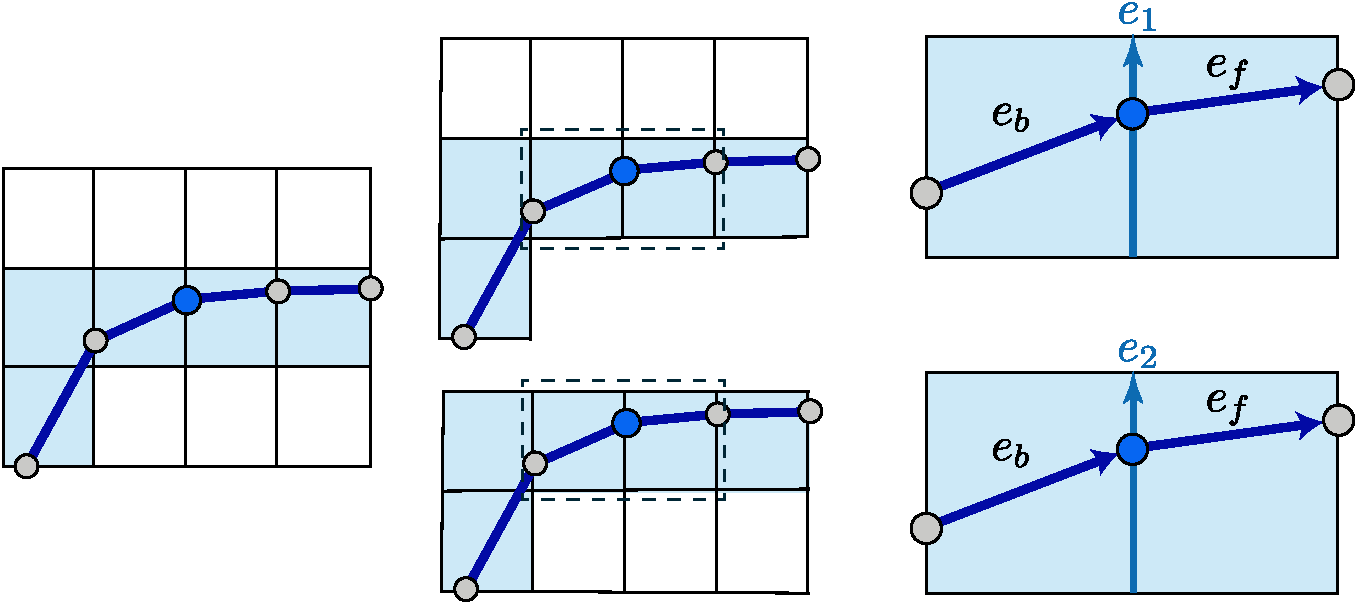
\includegraphics[width=\linewidth]{figures/osc_plane_discretization}
	\caption{Notation for edges in a discrete crease pattern. Left: a DOG net with a discrete crease curve. Center: Following \cite{rabi2018shape}, we represent creases by duplicating the quads that contain the crease curve, which results in different connected components, or patches. The positions of the vertices on the curve, i.e., its intersection points with the grid edges, are constrained to match on both patches. Right: Notation for a duplicated grid edge ($e^1, e^2$) intersecting the crease curve at the blue point(s), and the two crease edges $e_f,e_b$. }
	\label{fig:osc_plane_discretization}
\end{figure}

In the notation of \figref{fig:osc_plane_discretization}, the supporting plane constraint can be written as
\begin{equation} \label{eq:folding_const_normalized} 
\text{sgn}(\langle t^1,B\rangle) +  {sgn}(\langle t^2,B\rangle) = 0
\end{equation}
with 
\begin{equation} \label{eq:sign}
\text{sgn}(x) = \left\{
     \begin{array}{@{}r@{\thinspace}l}
       -1  &: \text{if } x < 0, \\
       0 &: \text{if } x = 0, \\
       1 &: \text{if } x > 0. \\
     \end{array}
   \right.
\end{equation}
%
Constraint \eqref{eq:folding_const_normalized} can be simplified by replacing $B$ with the non-normalized $\langle e_f \times e_b \rangle$. Furthermore, if one assumes an isometric deformation, it is possible to replace $t^1,t^2$ by the non-normalized edges $e^1,e^2$, arriving at:
\begin{equation} \label{eq:folding_const}
\text{sgn}(\langle e^1,e_f \times e_b \rangle) +  {sgn}(\langle e^2,e_f \times e_b\rangle) = 0.
\end{equation}
%
\OSH{I don't like ending a paragraph on an equation, looks incomplete. Say a sentence about how we use this constraint? Add it to the modeling system along with DOG constraints and continuity constraints for patch boundaries?}

\subsection{Discussion}
There are multiple equivalent characterizations for a folded crease over a curved folded surface. We now point out some key properties of our chosen discretization \eqref{eq:folding_const_normalized} and briefly discuss how these properties elude other possible constraint choices.

\paragraph{Suitable for homotopy based optimization methods} 
Our constraint is satisfied on a flat mesh. In this sense we consider a point along a curve with zero normal curvature as both folded and not folded.
 
\paragraph{Minimal and generally non-intrusive} 
Once a curved crease is folded on a piecewise DOG, one no longer needs to explicitly take care for it to stay folded. The effect of \equref{eq:folding_const} on an already folded surface is null. The discontinuity along the tangents caused by the folding implies that a folded crease remains folded under local deformations, and in order for it to become unfolded, one need to first flatten it, as this is the case for a piecewise smooth curved folded surface. It also captures the converse: a curved crease can only be folded when starting from a point with zero normal curvature \cite{more_on_paper}. \\

An alternative constraint for folding could be e.g.\ enforcing discontinuities along the tangents $t^1,t^2$, but this loses the feasibility of the flat models. Moreover, in the discrete case a minor discontinuity can still arise even though there is no fold, i.e., where \equref{eq:folding_const_normalized} is not satisfied, thus numerically giving the impression of a fold when visually there is none. Another option is to define folded configurations as those satisfying a similar but simpler smooth constraint:
%
\begin{equation} \label{eq:folding_const_smooth} 
\langle t^1,B\rangle + \langle t^2,B\rangle = 0.
\end{equation}
%
This condition is satisfied exactly in flat models and in any piecewise smooth curved folded surface, since tangent planes along a folded creased curve are reflections of each other w.r.t\ the osculating plane of the crease curve. However, this condition is not satisfied \emph{exactly} on every folded piecewise DOG (as evident by all models in this paper). An exception to this is the class of curved creases with zero torsion, in which case the folds are simply formed as a global plane reflection \cite{Mitani_ref}. Therefore, enforcing constraint \eqref{eq:folding_const_smooth} as a hard constraint is too restrictive in practice, while enforcing it softly creates a condition that, unlike the smooth case, does not vanish once a crease is folded and hence is not minimal in our sense.

\section{Folding angles and mountain-valley assignments} \label{sec:folding_angles_mountain_valley}
In this section we build tools to control a deformations folding angles and their direction, giving a designer more expressiveness and freedom. We first show how to constrain folding angles, i.e. the angles between the tangent planes around a crease, by constraining DOG tangent angles, resulting in a simple quadratic constraint. We then devise a tool to differentiate between mountain or valley folds. Our derivations work for both a curved and straight origami creases.

\subsection{Folding angle} A folding deformation can be seen as a rotation of tangent vectors around the tangent of a crease point. If a fold crease is a straight fold then the crease tangent is constant and so is the folding angle, while around a curved crease both the tangent and the folding angles often vary. In both cases if the folding angle at a given point is $\theta$, then tangents on both sides that are orthogonal to the crease tangent form an angle of $\theta$, while tangents that are parallel to the crease pattern remain parallel to each other. The following lemma shows the relation between an angle of tangents that are equal on a flat configuration and the folding angle (see \figref{fig:fold_angle_and_tangent_angles}): 
 \begin{lemma}  \label{lem:tangents_dihedral}
 Let $t_1,t_2$ be tangents on two sides of a crease curve at a given point that are equal on the flattened isometric developable surface. Let $t$ be the crease curve tangent at that point. Assuming the surface went through a curved folding isometric deformation and the folding angle at a given point along the crease is $\theta$ then the tangents satisfy:
\begin{equation} \label{eq:tangents_dihedral}
\langle t_1, t_2 \rangle = cos(\alpha)^2 + sin^2(\alpha) cos(\theta) \end{equation}
%4*cos(alpha/2)/(norm(e1)+norm(e2))
\end{lemma}
\begin{proof}{Let $\{t,n,b\}$ be the Frenet frame of the curved crease at the point. An angle $\alpha$ means that at the flat isometric configuration both tangents can be written as $cos(\alpha)t + sin(\alpha)n$. A folding angle of $\theta$ at a given point means that relative to the Frenet frame of the curve, tangents on one surface where rotated in angle $\frac{\theta}{2}$ around the crease's tangent $t$, while on the other surface they were rotated in an angle  $-\frac{\theta}{2}$. Thus w.l.o.g $t_1 = cos(\alpha)t + sin(\alpha)(cos(\frac{\theta}{2})n+sin(\frac{\theta}{2})b)$ and $t_2 = cos(\alpha)t + sin(\alpha)(cos(\frac{\theta}{2})n-sin(\frac{\theta}{2})b)$. The proof ends by computing $\langle t_1,t_2 \rangle$ and plugging in the trigonometric identity $cos(\theta) = cos^2(\frac{\theta}{2})-sin^2(\frac{\theta}{2})$.}\end{proof}

At \secref{sec:implementation} we show that under an isometric deformation and for a fixed dihedral angles, constraining dihedral angles using \eqref{eq:tangents_dihedral} can be written as linear constraints.

\begin{figure} [h]
	\centering
	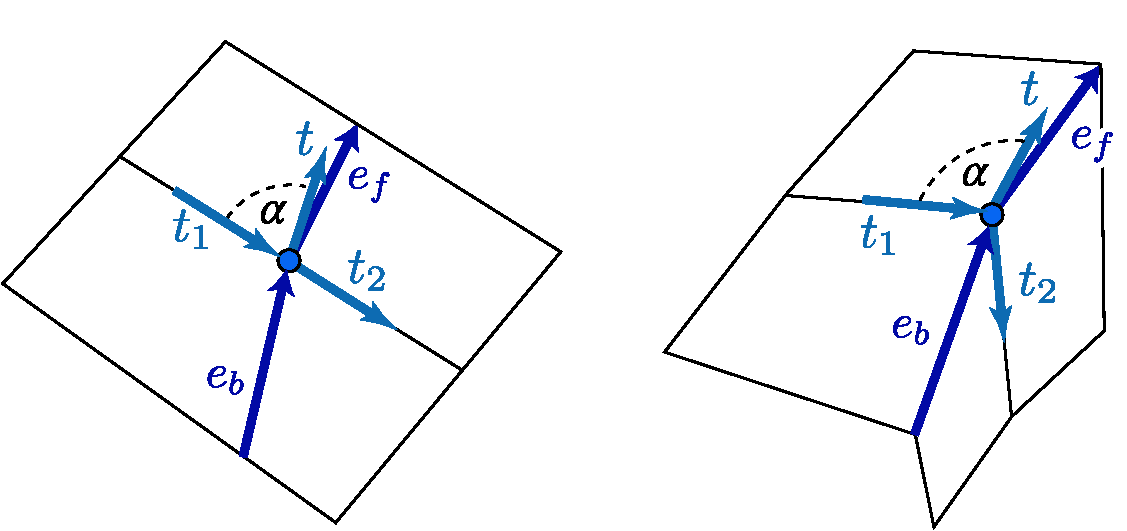
\includegraphics[width=0.7\linewidth]{figures/fold_angle_and_tangent_angles}
	\caption{Left: A flattened configuration of a curve (gray) with edges $e_f,e_b$ and its tangent $t$, forming an angle $\alpha$ with the DOG tangents $t_1,t_2$ which are equal. Right: A folded isometric configuration with a discontinuty between $t_1,t_2$. \lemmaref{lem:tangents_dihedral} shows the connection between the tangents angles and the folding angle $\theta$ in the smooth case, stating that $\langle t_1, t_2 \rangle = cos(\alpha)^2 + sin^2(\alpha) cos(\theta)$. }
	\label{fig:fold_angle_and_tangent_angles}
\end{figure}

\subsection{Mountain/Valley assignments} As mentioned, there are a few combinatorial degrees of freedom in choosing the type of fold, i.e. the choice of surfaces from each side of the curve (see \figref{fig:folding_combinatorics}). We follow \cite{demaine_lens} to distinguish between the two type of folded configurations in \figref{fig:folding_combinatorics} by calling one choice a \textit{Mountain} fold and the other a \textit{Valley} fold. We would like to emphasis that for straight folds this degree of freedom always exists, but around curved creases it often doesn't. In fact, in many crease patterns its often only possible to choose one Mountain/Valley (M/V) assignment, and the rest are determined by the propagation of the rulings leaving the only combinatorial degrees of freedom  as the choice to fold or not fold, as embedded in eq. \eqref{eq:folding_const_normalized}. For instance, in \cite{demaine_lens} the authors proved how segments on the convex side of a crease bend mountain/valley the same as the crease, while segments on the concave side of a crease bend mountain/valley opposite from the crease. This can be seen in \figref{fig:multiple_crease_patterns}, where the left crease pattern has a mountain and valley fold while the center one has only valleys.
  We distinguish between M/V folds by looking at whether a tangent of one surface is above or below the tangent plane of the second surface at the point of the crease, for a consistent choice of orientation. This can be achieved by the following constraint:
\begin{equation} \label{eq:mountain_valley_ineq}
\langle t_1, t \times t_2 \rangle \leq 0
\end{equation}
where $t$ is the tangent of the creases curve oriented, and $t \times t_2$ is the tangent plane of the surface with $t_2$ as a tangent vector. The orientation of $t$ determines whether a mountain or valley fold is chosen. By the cyclic property of the triple product \eqref{eq:mountain_valley} is also equal to $\langle t_2, t_1 \times t \rangle$.
Using the notation of figure \figref{fig:fold_angle_and_tangent_angles}, we discretize the tangent of the crease curve as $t = \frac{\|e_b\|e_f + \|e_f\|e_b}{\|\|e_b\|e_f + \|e_f\|e_b\|}$, which for a creased curve is the tangent to the point at the unique circle passing through three points, and is linear in the vertices under isometry.
To ease up notation in \secref{sec:implementation}, we reformulate \eqref{eq:mountain_valley_ineq} in an equivalent formulation with equalities by using the Heaviside step function:
\begin{equation} \label{eq:heaviside}
\text{H}(x) = \left\{
     \begin{array}{@{}l@{\thinspace}l}
       0  &: \text{if } x \leq 0, \\
       1 &: \text{if } x > 0. \\
     \end{array}
   \right.
\end{equation}
and write down the mountain valley condition as:
\begin{equation} \label{eq:mountain_valley}
H(\langle t_1, t \times t_2 \rangle) = 0
\end{equation}